\section{Background and Motivation}
\label{sec:background}

In this section we outline the process for defining a UML profile and the supporting graphical model editing facilities for the UML profile in Papyrus. 
This process typically involves the manual creation of a number of inter-related models and configuration files.
We highlight labour-intensive and error prone activities involved in the process that motivate the need of automatic generation of these artefacts.

\subsection{UML Profile}
A UML Profile in Papyrus is an EMF model that conforms to the UML Ecore metamodel. 
In order to create a new UML Profile, developers need to create instances of \textit{Stereotype, Property, Association}, etc. to create the elements of their domain specific modeling languages, and their properties and relationships among the elements.

Papyrus offers, among other choices, the mechanism of creating UML profiles using a \textit{Profile Diagram}. 
Users can use the palette provided in the UML Profile Diagram editor to
create all elements required to form a UML profile.
The properties of each element (e.g., data types of properties, multiplicity, navigability, etc.) can then be set using the properties view. 
In a profile, each \textit{stereotype} needs to extend a UML concept (hereby referred to as \textit{base element} or \textit{meta-element}). 
Thus, users need to define which meta-elements their stereotypes extend. 
This is achieved by importing the meta-elements and by adding appropriate extension links between their stereotypes and the meta-elements by using the tool provided in the palette.
The process of creating a UML profile can be repetitive and labour-intensive, depending on the size of the profile.
Having created a profile, users can then apply it to a UML model. 
Users typically create instances of UML meta-elements (e.g., UML::Class) and apply their stereotypes defined in their UML profiles. 
For example, if a stereotype extends the UML::Class meta-element, users can apply it to selected instances of UML::Class in their models. 
In this sense, the users are creating instances of the elements they define in their DSLs. 

One of the limitations of UML profiles in Papyrus is that links between stereotypes can be instantiated as edges in a diagram only if they extend a \textit{Connector} meta-element (e.g., UML::Association).  
For example, if ``Stereotype A'' refers to ``Stereotype B'' via an ``A\_to\_B'' reference, then in order to be able to draw this connection as an edge on the diagram, ``A\_to\_B'' should be created as a separate stereotype. 
These connector stereotypes do not hold any information about the stereotypes that they can connect, so users need to define such restrictions by manually writing OCL constraints to validate at least two things: 1) if the source and target nodes are of the correct type and 2) if the connector is in the correct direction (e.g., for ``A\_to\_B'', the edge should lead from ``Stereotype A'' to ``Stereotype B''. 
These constraints can be rather long and need to be manually written and customised for \textit{each} edge stereotype. This, as illustrated in Section~\ref{sec:constraints}, can also be a labour-intensive and error-prone process.

\subsection{Distributable Custom Graphical Editor}
With the UML profile created, users can apply it to UML diagrams. 
Users select a UML element (e.g., an instance of UML::Class) and manually apply a stereotype in the UML profile they define. 
A stereotype can only be applied to instances of the meta-elements they extend.
For example, a stereotype that extends the UML::Package meta-element in the profile cannot be applied to an instance of UML::Class. 
This task is arguably labour-intensive and repetitive. 
In addition, users typically need to remember the meta-element that each stereotype extends in their UML profile. 
%It is even more 
%problematic in scenarios where the profile was created by someone else. In 
%fact, except from using the profile in their local machine, users can 
%distribute it (all the needed information are stored in a file called 
%``model.profile.uml'') so it can be used by others. 

% Although the aforementioned manual creation and use of the profile sometimes covers all the needs of the stakeholders and includes trade-offs they are willing to take, it is usually the case that stakeholders require the definition of custom shapes for the stereotypes and/or a custom palette of stereotypes. The later is important if one thinks that in smaller profiles, users actually need to navigate through tenths of elements available in the default palette, to pick the one that should be used and apply the stereotype. 
To address this recurring concern, Papyrus offers at least three possible options for creating a custom palette which allows users to create UML elements and apply selected stereotypes on them in a single step. 
%Papyrus provides the facility to customise the palette for an open editor. 
In the first option, users can make use of the customisation facility to create their own palettes, and then specify what stereotypes should be instantiated for the creation tools in the palette.
Although this is an easy-to-use approach, it must be done manually every time a new diagram is created.
In addition, it cannot be shared in case the editor needs to be distributed to collaborators. 
%The first option involves customisation through a user interface where users add elements in the palette for their stereotypes. 
%Although this is an easy-to-use approach, it has to be done manually when a new diagram is created. 
The second option involves the manual definition of an XML-based palette configuration file which is automatically loaded every time the profile is applied to a diagram. 
This option however, is discouraged by Papyrus as it does not allow the full use of Papyrus functionality.
Furthermore, this option is based on a deprecated framework, and its use is not encouraged. 
The third option is to create a UML profile editor, which includes the manual creation of a number of inter-related models and artefacts, including a palette configuration model. 
Although this option provides a whole solution to create a UML profile editor, in the paper we illustrate that it is a labour-intensive and error prone process.

%\begin{figure}[ht]
%	\centering
%	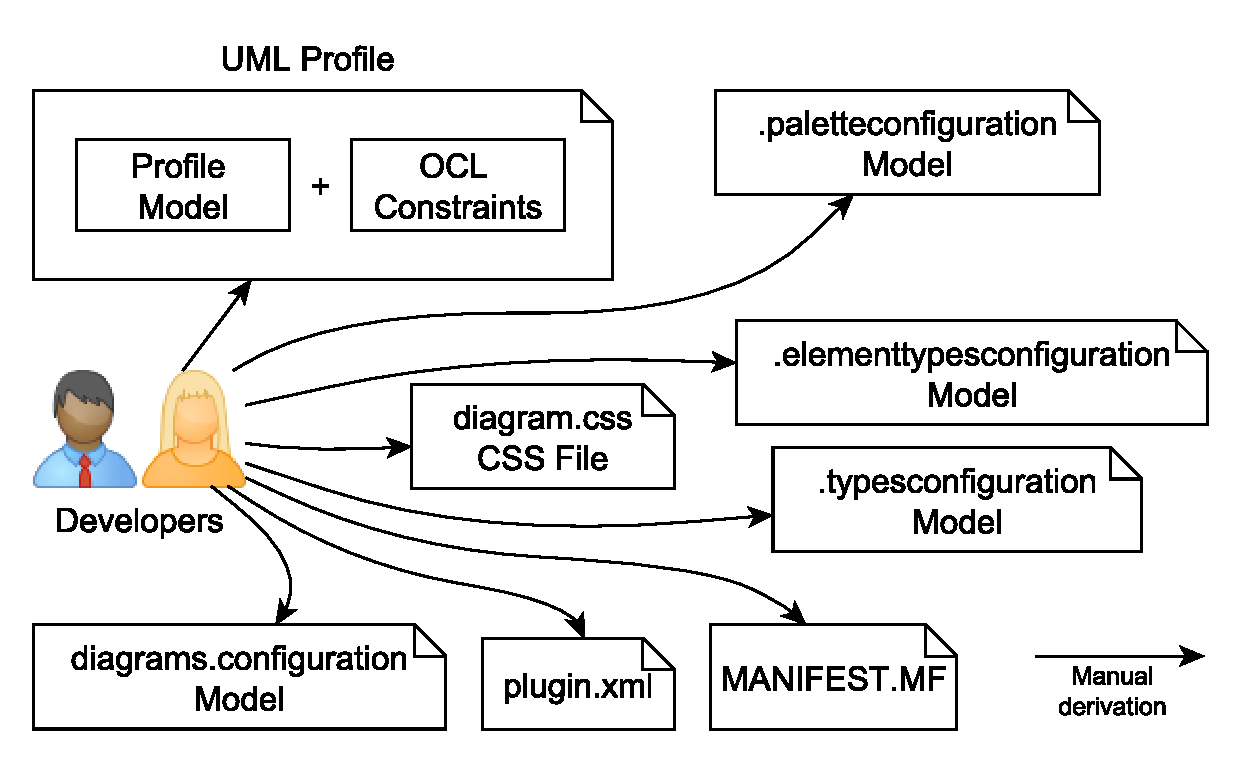
\includegraphics[width=1\textwidth]{diagrams/neededPapyrusFiles.pdf}
%	\vspace{-3mm}
%	\caption[]{Models/files developers need to write manually to 
%		develop a fully functional distributable Papyrus profile editor for Papyrus 2.0.}
%	\label{fig:neededPapyrusFiles}
%%	\vspace*{-3mm}
%\end{figure}

The definition of custom shapes for the instantiated stereotypes is another common requirement. 
In Papyrus, Scalable Vector Graphics (SVG) shapes can be bound to stereotypes during the profile creation process. 
However, to make these shapes visible, users need to set the visibility of the shape of \textit{each} stereotype to true. 
Although this is an acceptable trade-off, the users typically need to hide the default shapes by writing custom style rules in a Cascading Style Sheet (CSS), as by default the SVG shape bound to a stereotype overlaps with the default shape of the base meta-element.
The CSS can be written once but need to be loaded each time \textit{manually} on every diagram that is created. 

\begin{figure}[ht!]
	\centering
	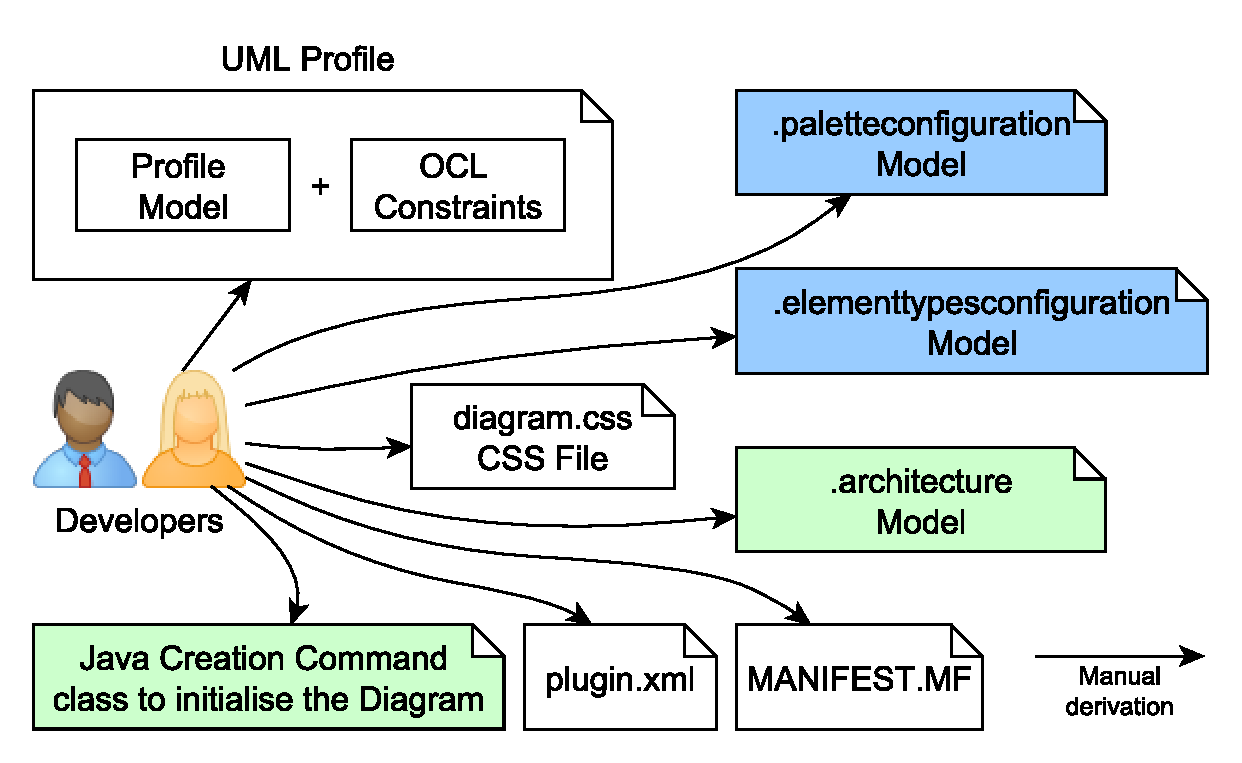
\includegraphics[width=1\textwidth]{diagrams/neededPapyrusFiles_new.pdf}
	\vspace{-3mm}
	\caption[]{Models/files developers need to write manually to 
		develop a fully functional distributable Papyrus profile editor for Papyrus 3.0+.}
	\label{fig:neededPapyrusFiles_new}

	%	\vspace*{-3mm}
\end{figure}

To create a distributable graphical editor that has diagrams tailored for the profile and to avoid all the aforementioned drawbacks, users need to create a number of inter-related models and files, and to implement extension points in an Eclipse plug-in project. 
To create a working UML profile editor in Papyrus, users typically need to create:
\begin{itemize}
	\item An Element Types Configuration model;
	\item A Palette Configuration model;
	\item A Cascading Style Sheet for customised styles;
	\item A Java Creation Command class to initialise the diagram;
	\item An Architecture model to describe the architecture of the editor;
	\item Plug-in related files for extensions and dependencies.
\end{itemize}

Figure~\ref{fig:neededPapyrusFiles_new} shows all the artefacts needed to be created for having a distributable Papyrus UML profile editor for Papyrus 3.0+\footnote{Metamodels for Element Types Configuration, Palette Configuration have been changed since our previous work (rendered in blue). 
The Architecture model and the Java Creation Command class are new concepts introduced in Papyrus 3.0 since our previous work (rendered in green).}.

Through our experiment (see Section~\ref{sec:evaluation}), we found out that it is difficult, if not impossible, to create these models without any working examples, taking also into account that the documentation of Papyrus provides limited useful insight in this matter.
%In addition, it is also a labour-intensive and error-prone process to migrate editors created based on Papyrus 2.0 to Papyrus 3.0+. 
%Developers typically need to create new Palette Configuration and Element Types Configuration models, as well as the new concepts such as the Architecture model.

Detailed discussions about the artefacts needed in order to create a UML profile editor are provided in Section~\ref{sec:implementation}.
A few hundred lines of code need to be written while tedious and repetitive tasks (e.g., model creation) should be done. 
This is backed by our studies in the evaluation, which is discussed in Section~\ref{sec:evaluation}.

This \textit{labour-intensive}, \textit{repetitive} and \textit{error-prone} process could be automated. 
In this paper, we present our tool - Jorvik, which uses a single-source input to automatically generate a UML profile and models/files mentioned above for the generation of a distributable UML profile graphical editor for Papyrus. 
%This approach is described in Section~\ref{sec:approach} that follows. 
